\section{Improvements IV: Evaluation and Software}
\label{sec:evalsw}

\subsection{Metrics (I11)}
\code{evaluation.classification\_metrics()} reports, for every model and seed:
\begin{itemize}
\item \textbf{Accuracy} and \textbf{balanced accuracy} (mean per-class recall).
\item \textbf{Macro-F1}: the unweighted mean of per-class F1. It is the CV selection criterion,
      because it penalises neglecting any class.
\item \textbf{MCC} (Matthews correlation): a single-number summary that stays informative under
      imbalance.
\item \textbf{ROC-AUC}. In binary mode it is computed from \code{decision\_function}, the raw SVM
      margin, rather than from Platt probabilities, so it reflects the model and not the
      calibration fold. In multiclass mode it is the macro one-vs-rest AUC from \code{predict\_proba}.
      The paper reported no multiclass AUC.
\item \textbf{False-alarm rate} (FAR): the fraction of BENIGN flows flagged as any attack.
      \textbf{Detection rate} (DR): the fraction of attack flows flagged as \emph{some} attack. These
      are the two numbers an IDS operator cares about. In multiclass mode DR ignores confusions
      between attack types, since an LDAP flow labelled MSSQL is still blocked.
\end{itemize}
Confusion matrices are stored for every seed.

\subsection{Repetition and significance (I7)}
\paragraph{Multiple seeds.} \code{--seeds 0 1 2 3 4} repeats the \emph{whole} pipeline (sampling,
split, preprocessing, tuning, test) with five different seeds and reports mean $\pm$ standard
deviation. With 400 test flows, one misclassification is 0.25 points, and the seed-to-seed
standard deviation is typically 0.2--1 point. Single-run differences of that size cannot be
interpreted.

\paragraph{McNemar's test.} For each seed, the QSVM and RBF-SVM predictions on the \emph{same}
test flows are compared with the exact McNemar test~\cite{mcnemar1947,dietterich1998}. Let $n_{01}$
be the number of flows only the QSVM gets right and $n_{10}$ the number only the RBF gets right.
Under $H_0$ (equal error rates), $n_{01}\sim\text{Binomial}(n_{01}+n_{10},\tfrac12)$, and the
two-sided exact binomial $p$-value is reported. Tables in Section~\ref{sec:results} give the number
of seeds (out of 5) with $p<0.05$.

\subsection{Kernel diagnostics}
For every run, \code{kernel\_diagnostics()} records, on the training Gram matrix:
\begin{itemize}
\item \textbf{Concentration}: mean and standard deviation of the off-diagonal entries. Values near
      0 with tiny spread indicate $K\approx I$.
\item \textbf{Centred kernel--target alignment}~\cite{cortes2012}:
      \begin{equation}
      A(K,Y)=\frac{\langle K_c, T_c\rangle_F}{\|K_c\|_F\|T_c\|_F},\qquad K_c=HKH,\ T=YY^\top,\ H=I-\tfrac1N\bm1\bm1^\top,
      \end{equation}
      where $Y$ is the one-hot label matrix. Alignment measures how well kernel similarity matches
      label similarity. It is computed for both the quantum and the tuned RBF kernel.
\item \textbf{Geometric difference} $g(K_\text{RBF}\|K_Q)$ (Eq.~\ref{eq:gd}) on a random subset of
      400 training points, with $\lambda=10^{-3}$, both kernels normalised to trace $N$.
\end{itemize}

\subsection{Software engineering}
\paragraph{Backward compatibility.} Every original CLI flag (\code{--csv}, \code{--samples},
\code{--mode}, \code{--sampling}, \code{--n-qubits}, \code{--n-reps}) keeps its meaning. The
public classes (\code{ZZFeatureMap}, \code{QuantumKernel}, \code{QSVM}) keep their names and
methods, including \code{compute\_kernel\_value}, \code{compute\_kernel\_matrix},
\code{build\_kernel\_circuit}, \code{predict\_proba} and \code{score}, plus a \code{QSVM.pca}
property. New behaviour is opt-out (\code{--legacy}, \code{--legacy-scaling},
\code{--keep-duplicates}, \code{--no-log}, \code{--no-tune}).

\paragraph{New CLI options.} \code{--kernel}, \code{--entanglement}, \code{--backend},
\code{--alpha}, \code{--C}, \code{--alphas}, \code{--Cs}, \code{--shots}, \code{--seeds},
\code{--features}, \code{--extra-baselines}, \code{--out-dir}, \code{--quiet}. See
Appendix~\ref{app:cli}.

\paragraph{Outputs.} Each run writes \code{results.json}, containing all arguments, per-seed metrics,
tuning tables, diagnostics, McNemar results and data bookkeeping (duplicates removed, overlap),
plus a 6-panel figure \code{results\_seed<k>.png} (Figure~\ref{fig:runfig}).

\paragraph{Tests.} \code{tests/test\_core.py} contains 19 \code{unittest} cases (standard library
only, since pytest is not installed in the venv), covering engine correctness against Cirq and
against the original code, kernel properties, leakage-freedom of preprocessing, loader
reproducibility and deduplication, the metric implementations, and an end-to-end toy problem.
They run in about 15\,s.

\paragraph{Benchmark suite.} \code{benchmark.py} defines nine experiments (speed, headline, ablation,
bandwidth, qubits, shots, architecture, features, samples). Each configuration is a call to
\code{main.main()} with a fixed argument list, its results go to
\code{outputs/benchmark/<experiment>/<config>/}, and finished configurations are skipped, so the
suite is resumable. \code{make\_figures.py} turns those JSON files into every figure and table in
this report. The numbers in Section~\ref{sec:results} are therefore regenerated from code, not
copied by hand.

\paragraph{Legacy preserved.} \code{legacy/} contains the original three files unchanged, so the
original program can still be run (\code{python legacy/main.py}) and compared.

\begin{figure}[H]
\centering
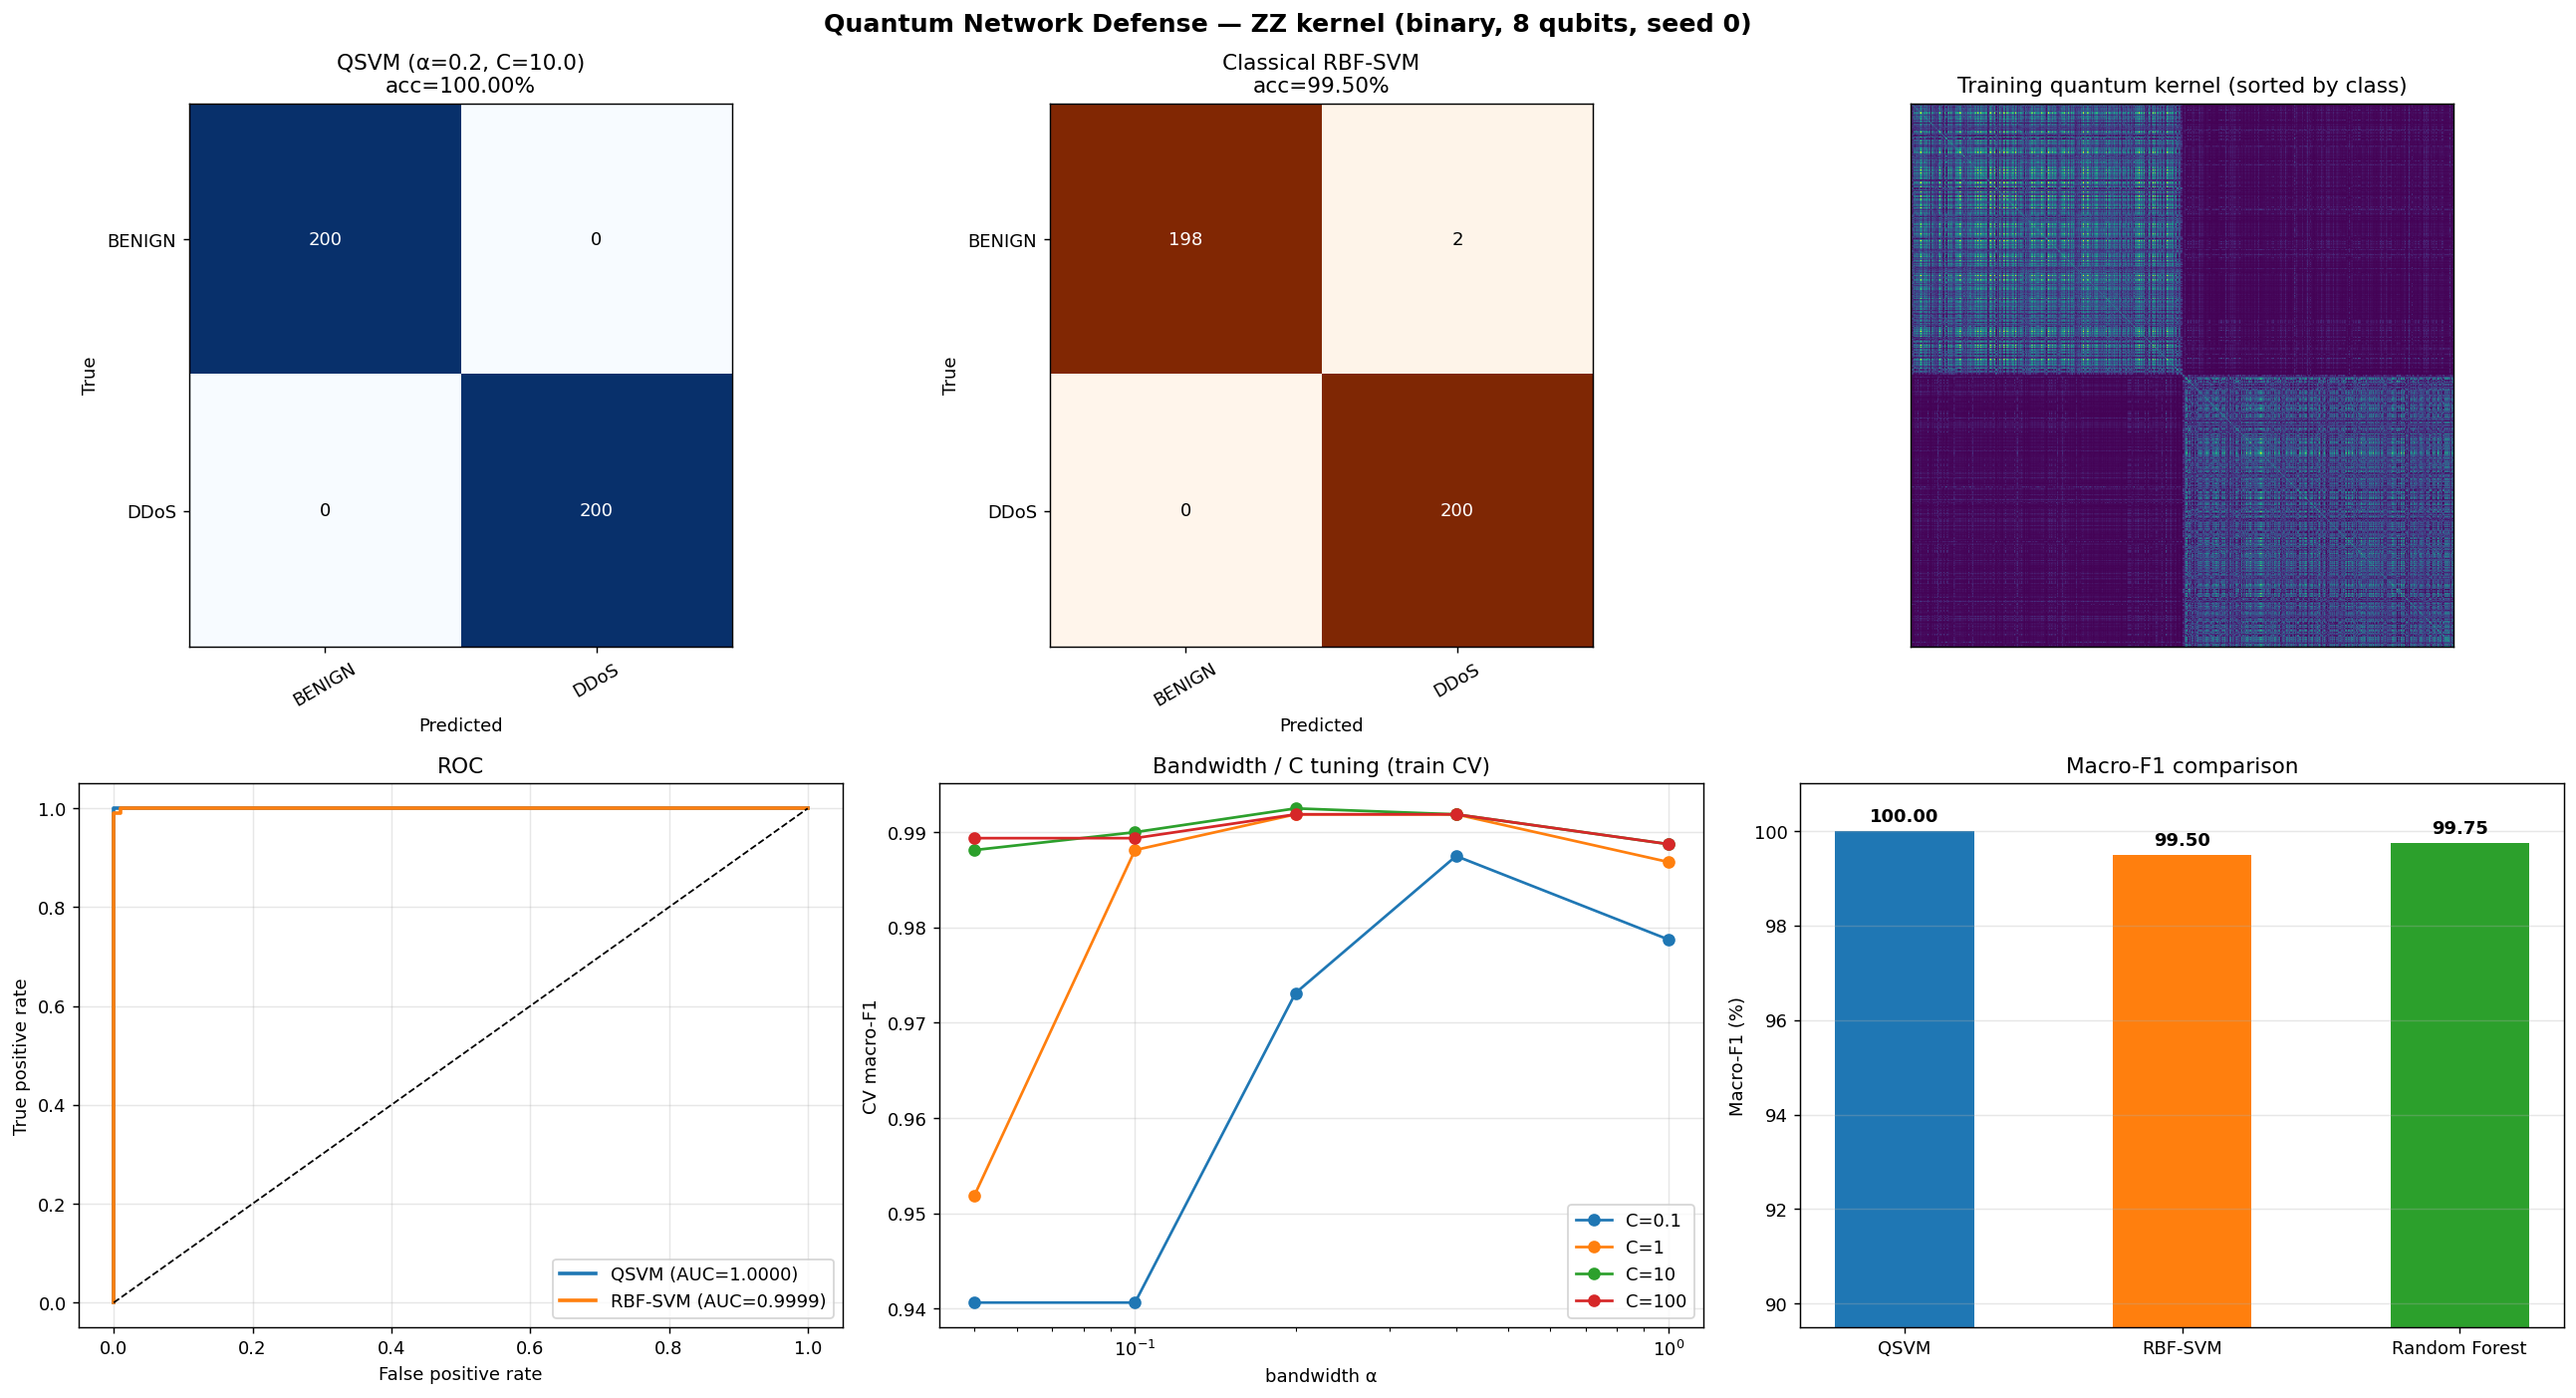
\includegraphics[width=\linewidth]{figures/run_binary.png}
\caption{Per-run figure written by \code{main.py} (binary task, ZZ map with 8 qubits and 2 reps,
improved protocol, seed 0). Top: QSVM and RBF confusion matrices, and the training quantum kernel
sorted by class (the block structure shows class-aware similarity). Bottom: ROC curves, the CV
tuning curves over $\alpha$ for each $C$, and macro-F1 of all models.}
\label{fig:runfig}
\end{figure}
